\documentclass[a4paper,11pt]{scrartcl}

\usepackage[margin=1in]{geometry}
\usepackage[scaled]{helvet}
\usepackage[T1]{fontenc}
\usepackage[utf8]{inputenc}
\usepackage{amsmath}
\usepackage{mathptmx}
\usepackage{courier}
\usepackage{graphicx}
\usepackage{ulem}
\usepackage{bookmark}
\usepackage{paralist}
\usepackage{ngerman}
\usepackage{fancyhdr}
\usepackage{float}
\usepackage{array}
\usepackage{lipsum}


\graphicspath{ {../img/} }
\renewcommand\familydefault{\sfdefault}




\pagestyle{fancy}
\fancyhf{}
\renewcommand{\headrulewidth}{0pt}
\fancyfoot[C]{
\includegraphics[width=\textwidth]{Polygon_gruen}\\ \thepage}
\setlength\parindent{0pt}

\rhead{
\includegraphics[width=\textwidth]{LogoHeader}}
\setlength\headheight{30pt}
\setlength\footskip{15pt}

\begin{document}
\renewcommand*{\arraystretch}{1.2}
\pagenumbering{gobble}
\begin{titlepage}
    \begin{center}
        \vspace*{1cm}\Huge
        \textbf{Projektplan}\par                
        \vspace{0.5cm}\LARGE        
        Software Engineering II\par           
        \vspace{2cm}
        
\includegraphics[width=0.5\textwidth]{OptimaLogo_long}\par   
        \vspace{1cm}
        \textbf{Projekttitel: BonoboBoard}\par        
        \vfill\Large   
        Jakob Hutschenreiter (1419081)\\Jiesen Wang (9839152)\\Nick Kramer (3122448)\\Patrick Küsters (2598689)\\Peter Moritz Hinkel (2783930)\par
        %\vspace{2cm}  
        %
\includegraphics[width=0.5\textwidth]{Bonobo_Logo}\par        
        \vspace{2cm}
        DHBW Mannheim\\
        \today     
    \end{center}
\end{titlepage}

\section*{Änderungshistorie}
\begin{table}[h]
	\begin{tabular}{@{} p{20mm} p{25mm} p{35mm} p{75mm}}
		\textbf{Revision} & \textbf{Datum} & \textbf{Autor(en)} & \textbf{Beschreibung}\\
		1.0 & 11.02.2022 & NK & A: Struktur\\
		1.1 & 11.02.2022 & NK,JW,JH,MH,PK & A: Ausarbeitung Inhalte\\
	\end{tabular}
\end{table}
\noindent
Abkürzungen: Hinzugefügt/Added (A), Änderung/Changed (C), Löschung/Deleted (D)
\vspace{2cm}
\tableofcontents
\newpage
\pagenumbering{arabic}

		%------------------------------------------------------------
		%-----  -----  ----- Begin actual content -----  -----  -----
		%------------------------------------------------------------
\section{Einleitung}\label{sec:einleitung}
Dieses Dokument befasst sich mit der Planung, Methodik und Organisation der Entwicklung des BonoboBoards von Optima Connect.

In einem ersten Schritt wird in Abschnitt \ref{sec:zeitliche-planung} ein Projektplan beschrieben, der aus dem verwendeten Projektmanagementtool Jira übernommen wurde.

In Abschnitt \ref{sec:methodik} wird auf die Methodik und Herangehensweise des Entwicklungsteams eingegangen. Die einzelnen Rollen, der iterative Entwicklungsprozess, sowie die individuelle Implementierung des Projekmanagementmodells Scrum werden hier erläutert.

Abschließend werden im Punkt \ref{sec:organisation} die Regeln für die Zusammenarbeit definiert und die verwendeten Tools, sowie deren Nutzung beschrieben. Ferner wird auf Guidelines für Code und den Entwicklungsprozess eingegangen.

\section{Zeitliche Planung}\label{sec:zeitliche-planung}

  \begin{figure}[H]
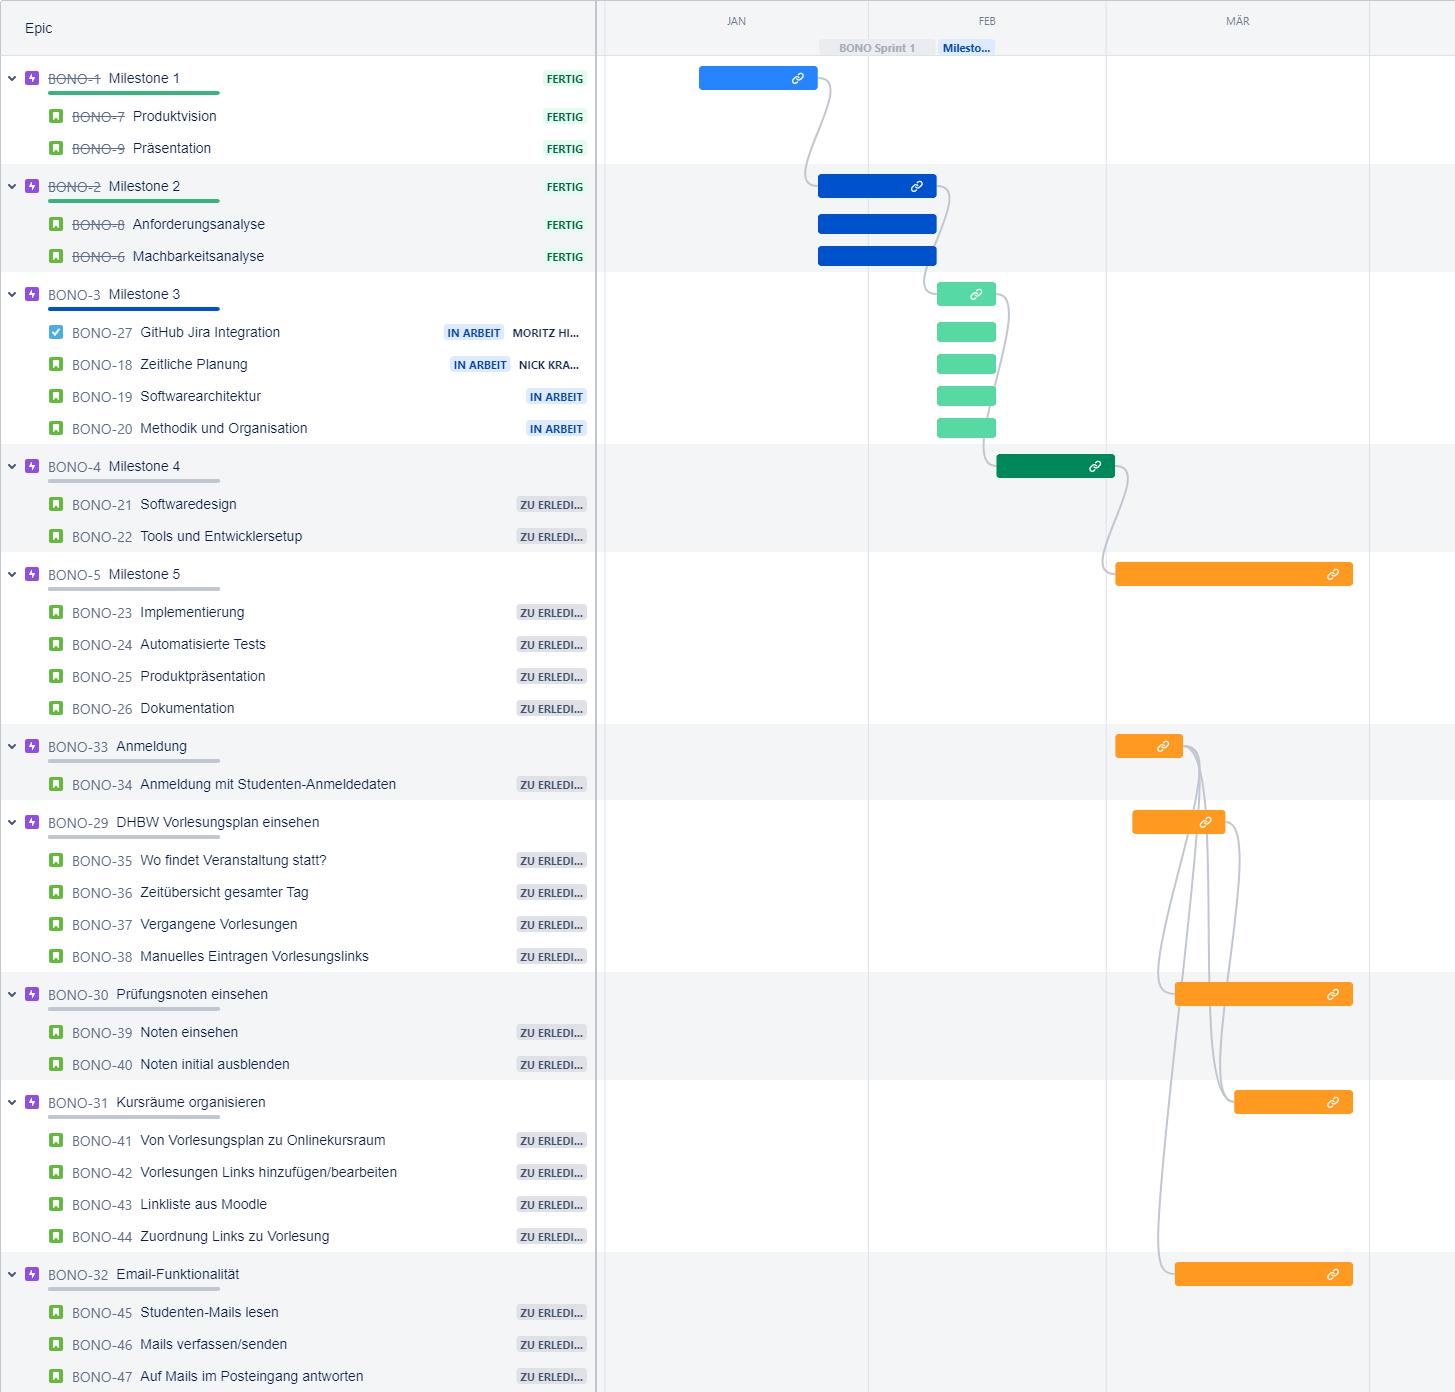
\includegraphics[width=\textwidth]{timeplan}
\caption{Zeitplanung mittels Atlassian Jira}
\label{img:Zeitplanung}
\end{figure}

Zur zeitlichen Planung unterteilen wir, wie in Abbildung \ref{img:Zeitplanung} dargestellt, die Abarbeitung des Projekts in Milestones, welche die Projektphasen darstellen und in Sprints abgearbeitet werden können. Dies liefert eine zeitliche Übersicht für alle Teammitglieder und zeigt transparent auf, wer an welchen Aufgaben arbeitet. Dadurch ist die individuelle Vorbereitung auf Teammeetings einfacher, da jeder vorab schon das derzeitige Arbeitsgebiet der Anderen kennt.

Die Roadmap wird auf der Plattform "`Jira"' gewartet. Der große Vorteil hierbei ist die Verknüpfung von Backlog, Sprint und Roadmap.

Im Zeitbereich des Milestone 5 findet die Implementierung des Projekts statt. Da hierzu Szenarien und zugehörige User Stories verfasst wurden, sind diese als Epics (Bsp: BONO-29 - DHBW Vorlesungsplan einsehen) und Stories (Bsp: BONO-35 - Wo findet Veranstaltung statt?) parallel zum fünften Milestone verankert.\\ 
Für den Vorlesungsplan ist keine Anmeldung nötig, daher kann diese Aufgabe parallel zum Handling der Anmeldung mit den DHBW-Zugangsdaten laufen. Ist die Implementierung der Anmeldung abgeschlossen, kann am Einsehen der Prüfungsnoten und der Email-Funktionalität gearbeitet werden.
Das Organisieren der Kursräume wird durch die Anmeldung und den DHBW-Vorlesungsplan blockiert und kann daher erst nach der Abarbeitung dieser Epics bearbeitet werden.
 

%- Diagramm mit einem Überblick zur Projektplanung
%- Projektplan sollte folgende Informationen enthalten:
%	o Meilensteine
%	o Projektphasen
%	o Zuordnung der Aufgabenpakete zu Projektphasen
%	o Zeitlicher Überblick von Beginn bis Ende des Projekts


\section{Methodik}\label{sec:methodik}
%- Schematische Darstellung / Beschreibung des Vorgehensmodells oder der individuellen Vorgehensweise 
%- Gründe für die Wahl der Vorgehensweise 
%- Art und Häufigkeit geplanter Teammeetings 
%- Methodik zur Verwaltung der Backlog-Items / Anforderungen
\subsection{Vorgehensmodell}
Unser Vorgehensmodell ist an die Scrum-Methode zum Projektmanagement angelehnt.
Scrum definiert 3 Rollen, einmal den Scrum Master, den Product Owner und die Entwickler.
Der Scrum-Prozess startet mit dem Product-Backlog, welches vom Product Owner geführt wird.
In diesem werden Produktanforderungen definiert, in Form von User Stories.
Diese Anforderungen werden in sogenannten Sprints umgesetzt.
Hierfür werden bestimmte Anforderungen ausgewählt und in das Sprint Backlog überführt.
Anschließend kommt es zur Planung des Sprintes (Sprint Planning),
an welchem alle drei Rollen teilnehmen. Das Sprint Ziel wird definiert und
als "`Definition of Done"' (DoD) festgehalten.
Der eigentliche Sprint hat eine Dauer von 1 bis 4 Wochen und täglich gibt es ein 15 minütiges Daily Scrum Meeting,
in welchem der Ist-Zustand der behandelten User Stories besprochen wird.
Nach Abschluss der Sprintdauer folgt das Sprint Review.
Alle nehmen wieder daran teil und der Product Owner überprüft,
inwiefern das entstandene Inkrement der DoD entspricht.
Bevor es nun zu einer neuen Iteration des Sprintes kommt,
gibt es noch die Sprint Retrospektive.
Dieses Meeting ist für die Entwickler gedacht und vom Scrum Master moderiert.
Es werden Stärken des Sprintes hervorgehoben und Schwächen aufgezeigt,
sodass im nächsten Sprint nicht die gleichen Fehler gemacht werden.

\subsection{Warum Scrum?}
\begin{itemize}
\item Kurze Kommunikationswege
\item Hohe Flexibilität/Agilität durch adaptives Planen
\item Hohe Effektivität durch Selbstorganisation
\item Kontinuierlicher Verbesserungsprozess / Iterativer Entwicklungsansatz
\item Hohe Transparenz (regelmäßige Meetings, Backlogs)
\item Zeitnahe Realisierung neuer Produkteigenschaften bzw. Inkremente
\item Kurzfristige Problem-Identifikation
\item Wenig Management-Overhead
\end{itemize}

\subsection{Wie nutzen wir Scrum?}
Wir nutzen die Scrum Methode, da eine agile Entwicklung für ein schnell und flexibel entstehendes Studentenprojekt als sinnvoll erachten werden kann. Hierbei wird von der klassischen Scrum-Struktur abgewichen. Sowohl Product Owner und Scrum Master sind im klassischen Sinne Personen, die nicht selbst entwickeln. Dies ist bei einer Gruppengröße von fünf Personen nicht sonderlich sinnvoll und verstößt zudem gegen die Anforderungen der Veranstaltung. \\
Unser Team besteht demnach aus einem Entwicklerteam, in welchem sich die unterschiedlichen Mitglieder einzelne Spezialisierungen gewählt haben. Diese verteilen sich wie folgt:
\begin{table}[H]
\begin{tabular}{|p{4.5cm}|p{8cm}|}
\hline
\textbf{Wer?} & \textbf{Funktion}\\ \hline
 Jakob Hutschenreiter &  Projekt-Lead und Backend\\ \hline
 Nick Kramer &  Backend und CI\\ \hline
 Jiesen Wang &   UI-Mockup und Django Frontend\\ \hline
 Moritz Hinkel &   Django Frontend\\ \hline
 Patrick Küsters &  Hopper\\ \hline
\end{tabular}
\end{table}

Die Verteilung der Arbeitspakete pro Sprint findet in gemeinsamer Auswahl nach dem Abschluss eines Sprints statt. Jede/jeder Entwickler*in wählt die gewünschten User Stories/Tasks selbstständig nach eigenen Stärken bzw. eigenem Interesse. Auf ein Daily Meeting wird verzichtet. Meetings finden immer auf Anfrage statt. 
\section{Organisation}\label{sec:organisation}
In diesem Abschnitt soll es darum gehen, wie die Entwicklung des BonoboBoard organisiert wird.  Wie die Zusammenarbeit zwischen den Entwicklern aussehen soll und welche Richtlinien und Werkzeuge verwendet werden.
\subsection{Regeln zur Zusammenarbeit}
Die Zusammenarbeit bei Optima Connect findet im Wesentlichen in drei Stufen statt: Teambesprechung, Entwicklung, Review.

Wenigstens einmal wöchentlich trifft sich das gesamte Team zu einem Discordmeeting, um die Entwicklungen der vergangenen Woche zu besprechen (wöchentliche Sprints) und offene Fragen zu klären. Offene Fragen werden im Vorfeld in einem OneNote Dokument gesammelt und dann der Reihe nach besprochen. 

Anschließend wird die Dokumentation der geleisteten Arbeit finalisiert und eventuell offene Tasks im Jira geschlossen, damit der Sprint beendet werden kann.

Im zweiten Teil des Meetings wird der neue Sprint geplant. Tasks erstellt und Konzepte besprochen, die für die Implementierung der jeweiligen Features relevant sind.

Bei Entscheidungen sind alle Teammitglieder gleichberechtigt, bei Uneinigkeiten wird ein Kompromiss ausgearbeitet. 
Als Plattform für die Visualisierung und für Notizen wird während den Meetings OneNote verwendet.

Nach erfolgter Planung beginnt die Entwicklungsphase in der die Mitarbeiter*innen einzeln, oder in Gruppen am Code arbeiten. Für die Gruppenarbeit wird Discord als Übertragungsmedium benutzt. Für jedes zu implementierende Feature, sowie für Fixes wird ein eigener Branch angelegt (siehe Guidelines). 

Sollen die Änderungen in das Projekt aufgenommen werden (main-branch) muss ein Pull-Request erstellt werden, der von wenigstens zwei Mitarbeiter*innen gesichtet und genehmigt werden muss. Sollten bei der Sichtung fragen auftreten, kann die Entwickler*in zu einer Erläuterung herangezogen werden.

\subsection{Projekt- und Entwicklungsguidelines}
\subsubsection{Style Guidelines}
Es wird sich während der Entwicklung an folgende Guidelines angelehnt: 
\begin{itemize}
\item PEP 8: https://www.python.org/dev/peps/pep-0008/
\item Google Python Style Guide: https://google.github.io/styleguide/pyguide.html
\item OOP Guide: https://wemake-python-stylegui.de/en/latest/pages/usage/violations/oop.html
\end{itemize}
In speziellen Fällen wird auf die Einhaltung verzichtet. 

\subsubsection{GitHub Team-Codex }
\begin{itemize}
\item Veränderungen werden nicht direkt auf dem "`main"'-Branch verrichtet. Änderungsübernahmen erfolgen nur über einen Merge-Request.  
\item Jeder Merge-Request benötigt mindestens zwei Genehmigungen von anderen Teammitgliedern. Nur die Person, die den Merge-Request gestellt hat, darf den Request auch nach den Genehmigungen mergen. 
\item Jeder erstellte Branch benötigt einen sprechenden Namen und muss einer der folgenden Kategorien zuordbar sein: 
\begin{itemize}
\item Core
\item Frontend 
\item Feature 
\item Bugfix 
\item Test  
\end{itemize}
\item[] Bsp: "`core/session\_handling\_request"', "`feature/docs\_faculty\_technic"', …
\end{itemize}

\subsection{Tools für das Projektmanagement/Organisation}

\begin{table}[H]
\begin{tabular}{|p{4cm}|p{8cm}|}
\hline
\textbf{Tool} &\textbf{Einsatzzweck} \\ \hline
Discord &  Austausch von Nachrichten, Virtuelle Meetings, Umfragen, Informationsmanagement\\ \hline
WhatsApp &  Austausch von Nachrichten\\ \hline
DropBox & Informationsmanagement \\ \hline
Google Kalender & Terminplanung   \\ \hline
Jira &  Aufgaben- und Projektmanagement, Prozessmanagement \\ \hline
Latex und Git &  Dokumente erstellen und bearbeiten \\ \hline
OneNote &  Informationsmanagement, Dokumentvorlagen erstellen und bearbeiten \\ \hline
Draw.io &  Diagramme erstellen und bearbeiten \\ \hline
Git und GitHub & Versionskontrolle und Repository-Verwaltung \\ \hline
Adobe XD & Ideen Entwicklung, Erstellung von Mockups \\ \hline
\end{tabular}
\end{table}

\section{Zusammenfassung}\label{sec:zusammenfassung}
Zusammenfassend lässt sich sagen, dass es sich bei der Entwicklung des BonoboBoards um ein Iteratives Projekt handelt, bei dem alle Teammitglieder sich gleichberechtigt, regelmäßig und selbständig einbringen. Die zeitliche Planung und Taskorganisiation wird im Milestone 5 (Entwicklung) in fünf Epics unterteilt, die bis auf einige Abhängigkeiten, weitestgehend parallel bearbeitet werden können.  Es kommen verschiedene Tools zum Einsatz, die die Planung und Entwicklung unterstützen.
		%------------------------------------------------------------
		%-----  -----  ------ End actual content ------  -----  -----
		%------------------------------------------------------------
\end{document}